\usetikzlibrary{decorations.text}
\usetikzlibrary{calc}
\usetikzlibrary{fit}
\usetikzlibrary{shapes}
\usetikzlibrary{arrows,positioning} 

%\begin{document}
\begin{figure}[h]
\begin{center}
\scalebox{1}{
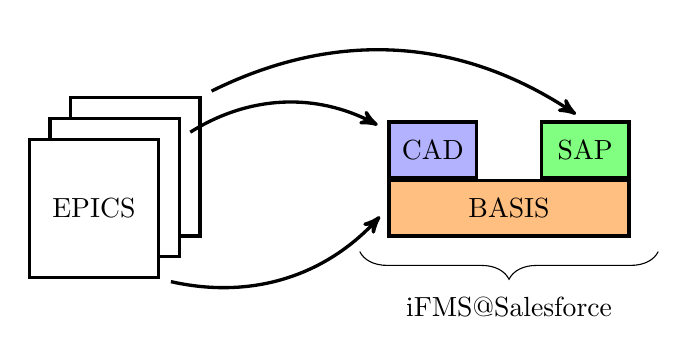
\begin{tikzpicture}[
    scale=5,
    pile/.style={thick, ->, >=stealth', shorten <=2pt, shorten
    >=2pt},
    punkt/.style={
           rectangle,
           draw=black, very thick,
           text width=8em,
           minimum height=2em,
           text centered},
    ]

\newcommand{\size}{1.5}
\coordinate (SW) at (0,0);
\coordinate (SE) at (\size,0);
\coordinate (NW) at (0,\size);
\coordinate (NE) at (\size,\size);

% axis
\newcommand{\cBasis}{orange!50}
\newcommand{\cCAD}{blue!30}
\newcommand{\cSAP}{green!50}

% iFMS@Salesforce
\node[punkt,fill=\cBasis] (BASIS) at (0,0) {BASIS};
\node[punkt,fill=\cCAD,text width=2.5em,anchor=south west] (CAD) at 
(BASIS.north west) {CAD};
\node[punkt,fill=\cSAP,text width=2.5em,anchor=south east] (SAP) at (BASIS.north 
east) {SAP};
;

% Klammer
\draw 
[decorate,decoration={brace,amplitude=10pt,mirror},xshift=-4pt,yshift=-200pt]
([yshift=-1pt,xshift=-2pt]BASIS.south west) -- 
([yshift=-1pt,xshift=2pt]BASIS.south east) node [black,midway,yshift=-20pt] 
{iFMS@Salesforce};

\coordinate (EPICS) at (-3em,0);
\newcommand{\epicsXShift}{0.15em}
\newcommand{\epicsYShift}{0.15em}
\node[punkt,text width=4em,minimum height=5em,fill=white] (E3) at ($ (EPICS) + 
(2*\epicsXShift,2*\epicsYShift) $) {};
\node[punkt,text width=4em,minimum height=5em,fill=white] (E2) at ($ (EPICS) + 
(\epicsXShift,\epicsYShift) $) {};
\node[punkt,text width=4em,minimum height=5em,fill=white] (EPICS) at (EPICS) 
{EPICS};

% Pfeile
\path[very thick, ->, >=stealth', shorten <=4pt, shorten >=4pt]
    (EPICS.south east) edge[bend right] node [right] {} (BASIS.west)
    (E2) edge[bend left] node [right] {} (CAD)
    (E3.north east) edge[bend left] node [left] {} (SAP.north);

\end{tikzpicture}
}
\caption{Schematische Darstellung der Zuordnung von Epics}
\label{fig:epics_to_components}
\end{center}
\end{figure}
